% Magic commands (just for TeXstudio)
% !TeX encoding = ISO-8859-1
% !TeX spellcheck = en_US

\documentclass[11pt,a4paper]{article}

\usepackage[latin1]{inputenc}
\usepackage{fancyhdr}
\usepackage{extramarks}
\usepackage{amsmath}
\usepackage{amsthm}
\usepackage{amsfonts}
\usepackage{tikz}
\usepackage[plain]{algorithm}
\usepackage{algpseudocode}
\usepackage{amssymb}
\usepackage{graphicx}
\usepackage{grffile}
\usepackage{mathtools}
\usepackage{enumerate}
\usepackage{tikz}
\usepackage{xifthen}
\usepackage{enumitem}
\usepackage{lipsum}
\usepackage{multicol}
\usepackage{listings}
\usepackage{my_commands}


%
% Basic Document Settings
%

\topmargin=-0.45in
\evensidemargin=0in
\oddsidemargin=0in
\textwidth=6.5in
\textheight=9.0in
\headsep=0.25in

\linespread{1.1}

% PDF-Links and Bookmarks
\usepackage{hyperref}
\usepackage{bookmark}

% New function cond
\DeclareMathOperator{\cond}{cond}

% Equal with def
\newcommand\myeq{\stackrel{\mathclap{\normalfont\mbox{def}}}{=}}

% Circled number 
\usepackage{tikz}
\newcommand*\circled[1]{\tikz[baseline=(char.base)]{
		\node[shape=circle,draw,inner sep=2pt] (char) {#1};}}

% This changes the default font family to sans-serif
\renewcommand{\familydefault}{\sfdefault}

% Framed to box a text (instead of fbox)
\usepackage{framed}
% \begin{framed} ... \end{framed}


% -------------------------------------------------------------------------------
\begin{document}
\section{New mathematical function}
For example \textit{cond}
\begin{verbatim}
\DeclareMathOperator{\cond}{cond}
\end{verbatim}
$\cond$\\
\textbf{Note:} Can be used only in preamble.

\section{For adding .py files}
\begin{verbatim}
% For adding .py files
\usepackage{listings}
% Example
\section*{�bung 3: \textit{LR-Zerlegung}}
{\footnotesize \lstinputlisting[language=Python,frame=single]
    {../../PycharmProject/Blatt_06/Aufgabe_3.py}}
\end{verbatim}

\section{New command / Redefine a command}
\begin{verbatim}
% New variable
\newcommand{\blatt}{8}
\textbf{Example: \blatt}

% Redfine variable
\renewcommand{\blatt}{9}
\textbf{Example: \blatt}
\end{verbatim}

% New variable
\newcommand{\blatt}{8}
\textbf{Example: \blatt}

% Redfine variable
\renewcommand{\blatt}{9}
\textbf{Example: \blatt}

\subsection{Command with multi arguments}
\begin{verbatim}
\newcommand{\tup}[2]{\ensuremath{\langle {#1}, {#2} \rangle}}
$\tup{test1}{test2}$
\end{verbatim}
\newcommand{\tup}[2]{\ensuremath{\langle {#1}, {#2} \rangle}}
$\tup{test1}{test2}$

\section{Cicled numbers (using tikz)}
\subsection{with aligment}
\begin{verbatim}
% Circled number 
\usepackage{tikz}
\newcommand*\circled[1]{\tikz[baseline=(char.base)]{
    \node[shape=circle,draw,inner sep=2pt] (char) {#1};}}
\circled{1} \circled{2} \circled{3}
\end{verbatim}

% Circled number 
%\usepackage{tikz}
%\newcommand*\circled[1]{\tikz[baseline=(char.base)]{
%		\node[shape=circle,draw,inner sep=2pt] (char) {#1};}}
\circled{1} \circled{2} \circled{3}

\subsection{out of aliegnment}
\begin{verbatim}
\textcircled{1}
\end{verbatim}
\noindent
\textcircled{1}

\section{Equal with def}
\begin{verbatim}
% Equal with def
\newcommand\myeq{\stackrel{\mathclap{\normalfont\mbox{def}}}{=}}
$ 1 \myeq 2 $
\end{verbatim}

% Equal with def
%\newcommand\myeq{\stackrel{\mathclap{\normalfont\mbox{def}}}{=}}
$ 1 \myeq 2 $

\section{Text over sign \texttt{stackrel}}
\begin{verbatim}
% Text over sign
$ A \stackrel{\text{text}}{\approx} B $
\end{verbatim}

% Text over sign
$ A \stackrel{\text{text}}{\approx} B $

\section{Overbrace with text}
\begin{verbatim}
$ \overbrace{a+b+c}^{d}  \quad \underbrace{a+b+c}_{d} $
\end{verbatim}
$ \overbrace{a+b+c}^{d}  \quad
 \underbrace{a+b+c}_{d}
$

\section{hrule}
\begin{verbatim}
\vspace{1ex}\hrule\vspace{1ex}
\end{verbatim}
\vspace{1ex}\hrule\vspace{1ex}

\section{Font}
\begin{verbatim}
% This changes the default font family to sans-serif
\renewcommand{\familydefault}{\sfdefault}
\end{verbatim}

% This changes the default font family to sans-serif
\renewcommand{\familydefault}{\sfdefault}

\section{Multi line comment}
\begin{verbatim}
\iffalse
\dots
\fi
\end{verbatim}

\section{Color}
\begin{verbatim}
{\color{red} colored text!!}
\end{verbatim}

{\color{red} colored text!!}

\section{Symbolic footnotes}
\begin{verbatim}
% Symbolic footnotes
\renewcommand{\thefootnote}{\fnsymbol{footnote}}
test\footnote{test}
\end{verbatim}
% Symbolic footnotes
\renewcommand{\thefootnote}{\fnsymbol{footnote}}
test\footnote{test}\\

Other options: \begin{verbatim}
\arabic, \Roman, \roman, ...
\end{verbatim}
See \href{https://www.sharelatex.com/learn/Footnotes}{sharelatex footnotes}

\section{Hyperref PDF-Links}
\begin{verbatim}
Test\label{test}
Go to \ref{test}
\end{verbatim}

Test\label{test}\\
Go to \ref{test}\\
To generate \textbf{PDF-bookmarks} for each section click the Rebuild button three times to generate link files and update references.\\
\textbf{Note:} sections must be numbered.\\
Links:\\
See more at \href{	ftp://ftp.ctan.org/tex-archive/macros/latex/contrib/oberdiek/bookmark.pdf}{Bookmarks PDF}\\
See more at \href{https://en.wikibooks.org/wiki/LaTeX/Hyperlinks}{Wikibooks \LaTeX - Hyperref}\\

\section{Supperpress sectionnumbering}
No need to write \texttt{section*} each time to avoid section numbering.

\begin{verbatim}
% Supperpress sectionnumbering
\makeatletter
\renewcommand\@seccntformat[1]{}
\makeatother
\end{verbatim}

\section{Lists}
\subsection{With letters}
\renewcommand{\theenumi}{\alph{enumi}}
\begin{verbatim}
\renewcommand{\theenumi}{\alph{enumi}}
\end{verbatim}

\begin{enumerate}
	\item first
	\item second
	\item third
\end{enumerate}

\section{Framed}
\begin{verbatim}
\begin{framed}
    framed text using framed package
\end{framed}
\end{verbatim}

\begin{framed}
	framed text using framed package
\end{framed}

\section{Cases}
\begin{verbatim}
\begin{cases}
    math & math \\
    math & math
\end{cases}
\end{verbatim}

Example:\\
$c'':E\rightarrow \mathbb{R}$ mit $c''(e) = 
\begin{cases} 
2c(e) &, \text{falls } e = (v,w) \text{ mit } v \in S, w\in V \backslash S\\
c(e) &, \text{sonst}
\end{cases}$

\noindent
\textbf{Note:} only one alignment symbol \& is allowed in each case\\
\textbf{Tip:} use spacing like quad before case condition

\section{Include another latex file}
\begin{verbatim}
Hi from another file :P
\end{verbatim}

Hi from another file :P

\textbf{Note:} using \texttt{include} instead of \texttt{input} will generate a new page.

\section{If with \texttt{xifthen} packge}
\begin{verbatim}
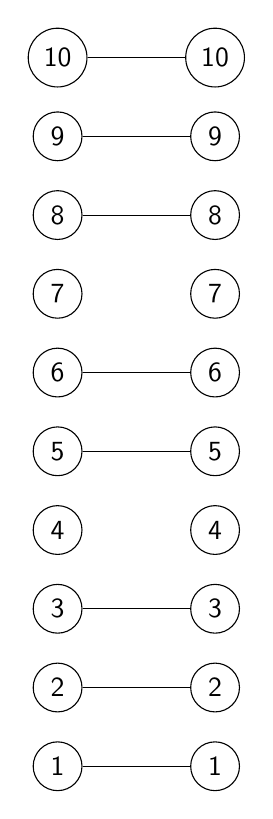
\begin{tikzpicture}
\foreach \x in {1,...,10}
{ \node[circle,draw] (\x 1) at (0,\x) {\x};
\node[circle,draw] (\x 2)at (2,\x) {\x};
\ifthenelse{\NOT \x = 4 \AND \NOT 7 = \x}{\draw (\x 1) -- (\x 2);}{}
}
\end{tikzpicture}
\end{verbatim}

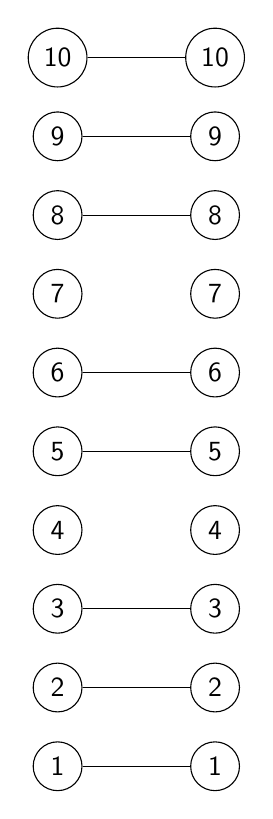
\begin{tikzpicture}
\foreach \x in {1,...,10}
{ \node[circle,draw] (\x 1) at (0,\x) {\x};
	\node[circle,draw] (\x 2)at (2,\x) {\x};
	\ifthenelse{\NOT \x = 4 \AND \NOT 7 = \x}{\draw (\x 1) -- (\x 2);}{}
}
\end{tikzpicture}

\section{Better graphics package for \texttt{includegraphics}}
Like avoid showing file name in graph\\
Solve space in filename issue\\
\texttt{\\usepackage\{grffile\}}

\section{Indent env.}
\begin{verbatim}
\usepackage{enumitem}

\setlist[description]{leftmargin=\parindent,labelindent=\parindent}
left aligned text
\begin{description}
    \item[One] first item
    \item[Two] second item
    \item[Three] third item
\end{description}
\end{verbatim}

\noindent
\setlist[description]{leftmargin=\parindent,labelindent=\parindent}
left aligned text
\begin{description}
	\item[One] first item
	\item[Two] second item
	\item[Three] third item
\end{description}

\section{Sample TikZ Diagram}
\begin{verbatim}
\tikzset{>=stealth}
    \tikzset{every node/.style={distance=.3cm,draw,circle,fill=none}}
    \tikzset{label/.style={draw=none,rectangle,fill=none}}
    \begin{center}
    \begin{tikzpicture}[->]
        % Nodes
        \node (a) at (0,0) {$a$};
        \node (b) at (2,2) {$b$};
        \node (c) at (2,0) {$c$};
        \node (d) at (2,-2) {$d$};
        \node (e) at (4,0) {$e$};
        % Edges
        \draw (a) to node [label,above] {$1$} (b);
        \draw (a) to node [label,above] {$2$} (c);
        \draw (a) to node [label,above] {$3$} (d);
        \draw (d) to node [label,right] {$-3$} (c);
        \draw (b) to node [label,above] {$1$} (e);
        \draw (c) to node [label,above] {$1$} (e);
    \end{tikzpicture}
\end{center}
\end{verbatim}

\tikzset{>=stealth}
\tikzset{every node/.style={distance=.3cm,draw,circle,fill=none}}
\tikzset{label/.style={draw=none,rectangle,fill=none}}
\begin{center}
	\begin{tikzpicture}[->]
	% Nodes
	\node (a) at (0,0) {$a$};
	\node (b) at (2,2) {$b$};
	\node (c) at (2,0) {$c$};
	\node (d) at (2,-2) {$d$};
	\node (e) at (4,0) {$e$};
	% Edges
	\draw (a) to node [label,above] {$1$} (b);
	\draw (a) to node [label,above] {$2$} (c);
	\draw (a) to node [label,above] {$3$} (d);
	\draw (d) to node [label,right] {$-3$} (c);
	\draw (b) to node [label,above] {$1$} (e);
	\draw (c) to node [label,above] {$1$} (e);
	\end{tikzpicture}
\end{center}

\section{Generate ipsum dummy text}
See more \href{http://texblog.org/2011/02/26/generating-dummy-textblindtext-with-latex-for-testing/}{textblog}
\begin{verbatim}
\usepackage{lipsum}
\lipsum
\lipsum[x]
\lipsum[x-y]
\end{verbatim}
\lipsum[1] % 1 Paragraph
%\lipsum[1-3] % Between 1 and 3 parahraphs

\newpage
\section{Force a column break in \texttt{multicols}}
See \href{http://tex.stackexchange.com/questions/8683/how-do-i-force-a-column-break-in-a-multi-column-page}{Stakexchange}\\
\begin{verbatim}
\usepackage{multicol}

\begin{multicols}{2}
    \lipsum[1]	
\vfill
\columnbreak
    \lipsum[1-2]
\end{multicols}
\end{verbatim}

\begin{multicols}{2}
	\lipsum[1]
	\vfill
	\columnbreak
	\lipsum[1-2]
\end{multicols}

\newpage

\section{Make your own package}
Write your own command such as \texttt{\textbackslash newcommand} or \texttt{\textbackslash newenvironment} in their own \texttt{.sty} file (example \texttt{my\_commands.sty}) and then use it in your document \texttt{\textbackslash usepackage\{my\_commands\}}.
\\
\\
Example:
\begin{framed}
\begin{lstlisting}[language=TeX]
\newcommand{\leftright}[2]{
	\begin{flushleft}
	#1
		\begin{flushright}
		#2
		\end{flushright}
	\end{flushleft}
}
\end{lstlisting}
\end{framed}
Result:
\begin{framed}
	\begin{lstlisting}[language=TeX]
	\leftright{left}{right}
	\end{lstlisting}
\end{framed}
\leftright{left}{right}

\section{Bibliography}
Source \href{https://www.sharelatex.com/learn/Bibliography_management_in_LaTeX}{Bibliography management in LaTeX}

\begin{verbatim}
	\cite{latexcompanion}
	
	\bibliographystyle{unsrt}
	\bibliography{sample}
\end{verbatim}

For computer science papers use \verb|\bibliographystyle{ieeetran}|

This is an example of BibTeX using in bibliography management. Three items 
are cited: \textit{The \LaTeX\ Companion} book \cite{latexcompanion}, the Einstein
journal paper \cite{einstein}, and the Donald Knuth's website \cite{knuthwebsite}. 
The \LaTeX\ related items are \cite{latexcompanion,knuthwebsite}. 

\bibliographystyle{unsrt}
\bibliography{sample}

\subsection{Show all bib entries without cite command}
Use: \verb|\nocite{*}|

\section{Verbatim environment}
\begin{itemize}
\item Environment
\begin{verbatim}
	\begin{verbatim}
	...
\end{verbatim}

\item Inline
\begin{verbatim}
	\verb|...|
\end{verbatim}

\end{itemize}

\section{Create a pdf document exactly as big as the content}
Use the \verb|standalone| package.\\
Example:
\begin{verbatim}
\documentclass{standalone}
\usepackage[utf8]{inputenc}
\usepackage{amsmath}
\usepackage{amsfonts}
\usepackage{amssymb}
\usepackage{graphicx}

\begin{document}
$
a+b
$
\end{document}
\end{verbatim}


\end{document}